\documentclass[a4paper]{article}
\usepackage[utf8]{inputenc}
\usepackage[T1]{fontenc}
\usepackage{amsmath}
\usepackage{amssymb}
\usepackage{bm}
\usepackage{hyperref}
\usepackage{xcolor}
\hypersetup{
    colorlinks,
    linkcolor={red!50!black},
    citecolor={blue!50!black},
    urlcolor={blue!80!black}
}
\usepackage{parskip}
\usepackage{float}
\usepackage{graphicx}
\usepackage{listings}
\lstset{language=Matlab, frame=single, breaklines=true,numbers=left, keywordstyle=\color{blue},rulecolor=\color{black},commentstyle=\color{gray}}
\usepackage[a4paper]{geometry}
\usepackage{cleveref}
\usepackage{todonotes}

\renewcommand\thesubsection{Problem \thesection\alph{subsection}}



\title{Linear Systems TTK4115 - Boat lab}
\author{
  Alex Danielsen-Haces -- 764088 \and
  Sindre Hansen -- 732719 \and
  Daniel Nakken -- 740939}
\date{November 2016}

\begin{document}

\begin{titlepage}
    \maketitle
    \rule{\linewidth}{0.5mm}
    \begin{figure}
    \centering
    
\includegraphics[width=0.5\textwidth]{images/logontnu_eng}
    \end{figure}
    \thispagestyle{empty}
\end{titlepage} 
%\section*{Table of contents}
\tableofcontents
\thispagestyle{empty} %Avoid page numbering on the table of contents
\newpage
\setcounter{page}{1}
\section{Identification of the boat parameters}
\subsection{Problem a}
Using the following state equations in the problem description \cite{assignment}
%
\begin{align*}
    \dot{\psi} &= r \\
    \dot{r} &= -\frac{1}{T}*r + \frac{K}{T}(\delta - b) \\
    \dot{b} &= w_b
\end{align*}
%
It is shown that $\dot{r} = \ddot{\psi}$ and assuming no disturbances and that b starts at 0, b will
always equal 0 since $\dot{b}$ = 0. Therefore:
%
\begin{align*}
    \ddot{\psi} &= -\frac{1}{T}*\psi + \frac{K}{T}\delta \\
    &\mathcal{L}\rightarrow  \\
    \Psi(s)s^2  &= -\frac{1}{T}\Psi(s)s + \frac{K}{T}\Delta(s) \\
\end{align*}
%
Rearranging this leads to:
\begin{equation}
    H(s) = \frac{\Psi(s)}{\Delta(s)} = \frac{K}{Ts^2 + s}
\end{equation}

\subsection{Problem b}
In order to measure the Nomoto time and gain constants T and K, the model is run with input sine waves
of amplitude one and frequencies $\omega = 0.005$ and $\omega = 0.05$. The amplitude of the output sine
waves are measured and these values correspond to $H(j\omega)$. This produces the following two
equations:

\begin{align*}
    H(0.005j) &= \left|\frac{K}{T(0.005j)^2 + 0.005j}\right| = 63.9575 \\
    H(0.005j) &= \left|\frac{K}{T(0.05j)^2 + 0.05j}\right| = 1.518
\end{align*}

Rearranging the equations results in the following values for T and K:

\begin{align*}
    T &= 85.6697 \\
    K &= 0.173945
\end{align*}

\begin{figure}[ht]
    \centering
    \begin{minipage}[b]{0.48\textwidth}
        \includegraphics[width=\textwidth]{"images/1b-omega_lik_0005"}
        \label{fig:1b-omega=0.0005}
        \caption{Heading over time ($\omega = 0.0005$)}
    \end{minipage}
    \hfill
    \begin{minipage}[b]{0.48\textwidth}
        \includegraphics[width=\textwidth]{"images/1b-omega_lik_005"}
        \label{fig:1b-omega=0.005}
        \caption{Heading over time ($\omega = 0.005$)}
    \end{minipage}
\end{figure}

\subsection{Problem c}
It is far more difficult to get good estimates of the boat parameters with waves and measurement noise
turned on. While easier with a lower frequency of the input signal, the accuracy of the estimates is not
satisfactory. With more samples it would be possible to average the results and get better estimates for
T and K. 

\begin{figure}[ht]
    \centering
    \begin{minipage}[b]{0.48\textwidth}
        \includegraphics[width=\textwidth]{"images/1c-omega_lik_0005"}
        \label{fig:1c-omega=0.0005}
        \caption{Heading over time ($\omega = 0.0005$)}
    \end{minipage}
    \hfill
    \begin{minipage}[b]{0.48\textwidth}
        \includegraphics[width=\textwidth]{"images/1c-omega_lik_005"}
        \label{fig:1c-omega=0.005}
        \caption{Heading over time ($\omega = 0.005$)}
    \end{minipage}
\end{figure}

\subsection{Problem d}
\todo[inline]{Explain the double amplitude figure}
The model closely follows the simulated physical system, and is thus a good approximation.

\begin{figure}[ht]
    \centering
    \begin{minipage}[b]{0.48\textwidth}
        \includegraphics[width=\textwidth]{"images/1d-dobbel_amplitude"}
        \label{fig:1d-dobbel_amplitude}
        \caption{Heading over time with double amplitude}
    \end{minipage}
    \hfill
    \begin{minipage}[b]{0.48\textwidth}
        \includegraphics[width=\textwidth]{"images/1d-riktig_amplitude"}
        \label{fig:1d-riktig_amplitude}
        \caption{Heading over time withe correct amplitude}
    \end{minipage}
\end{figure}
\newpage
\section{Identification of wave spectrum model}
\subsection{Problem a}
The MATLAB function \texttt{pwelch} calculates an estimate of the power spectral density PSD through
dividing the signal $\psi_w$ into K overlapping blocks multiplied by a windowing function, and finding an
estimate for the periodogram \todo{What is this word?} of each one.

\begin{figure}[h]
    \centering
    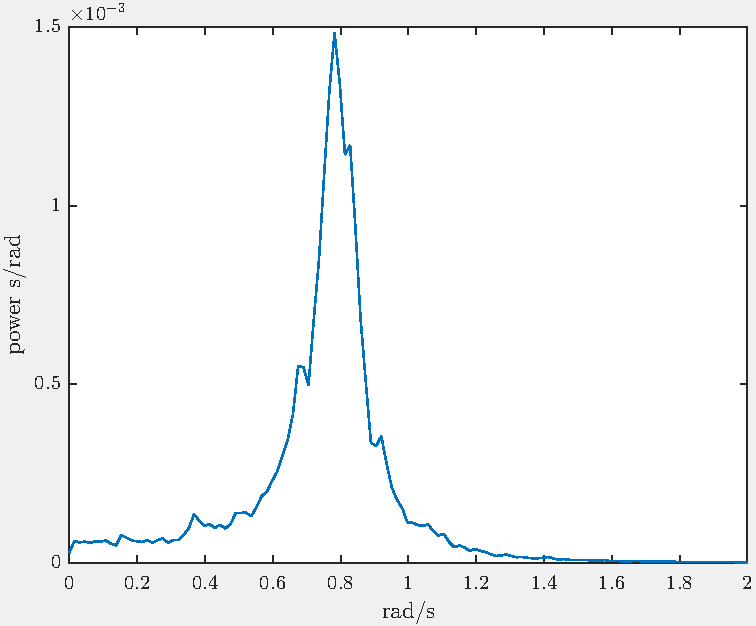
\includegraphics[width=0.5\textwidth]{images/2a-welchPSDestimate}
    \caption{Welch PSD estimate}
    \label{fig:2a-welchPSDestimate}
\end{figure}

\subsection{Problem b}
Using the following state equations in the problem description \cite{assignment}

\begin{align*}
    \xi_w &= \psi_w \\
    \dot{\psi}_w &= -\omega^2_0\xi_w - 2\lambda\omega_0\psi_w + K_ww_w
\end{align*}

the transfer function between $w_w$ and $\psi_w$ can be found.

Replacing $\xi_w$ with $\int\psi_w$ and taking the Laplace transform leads to:
\begin{align*}
    \Psi_w(s)s &= -\omega^2_0\Psi_w(s)\frac{1}{s} - 2\lambda\omega_0\Psi_w(s) + K_wW_w(s)
\end{align*}

Rearrange terms to get the transfer function:
\begin{align*}
    \frac{\Psi_w(s)}{W_w(s)} &= \frac{K_ws}{s^2 + 2\lambda\omega_0s + \omega^2_0}
\end{align*}

To find the Power Spectral Density function of S

\begin{align*}
    P_{\Psi_w}(\omega) &= E(\left|\Psi_w(s)\right|^2)|_{s=j\omega} \\
    &= E\left(\left|\frac{K_ws}{s^2 + 2\lambda\omega_0s + \omega^2_0}w_w(s)\right|^2\right)|_{s=j\omega} \\
    &= \frac{K_ws}{s^2 + 2\lambda\omega_0s + \omega^2_0}|_{s=j\omega} E(\left|w_w(s)\right|^2) \\
    &= K_w^2\frac{\omega^2}{\left|-\omega^2+\omega^2_0+2\lambda\omega_0\omega\right|^2} \\
    &= \frac{K_w^2w^2}{w^4+(4\lambda^2-2)w_0^2w^2+w_0^4}
\end{align*}

\subsection{Problem c}

$\omega_0 = 0.7823$, found through finding where the max of pxx$/2\pi$ is in the x-axis. This is the resonant 
frequency and the point where ???? $\psi_\omega$ correlates the most with itself.

\subsection{Problem d}
$\sigma^2$, the peak value of = 0.0015$
To fit $\lambda$, the MATLAB function \texttt{lsqcurvefit} was used. It finds $\lambda$ by minimizing an error
function between the target data $S_{\psi_\omega}(\omega)$, and the fitted function $P_{\psi_\omega}(\lambda, \omega)$ (forklar nøyere?). $\lambda$ was found to be 0.0827.

\begin{figure}[ht]
    \centering
    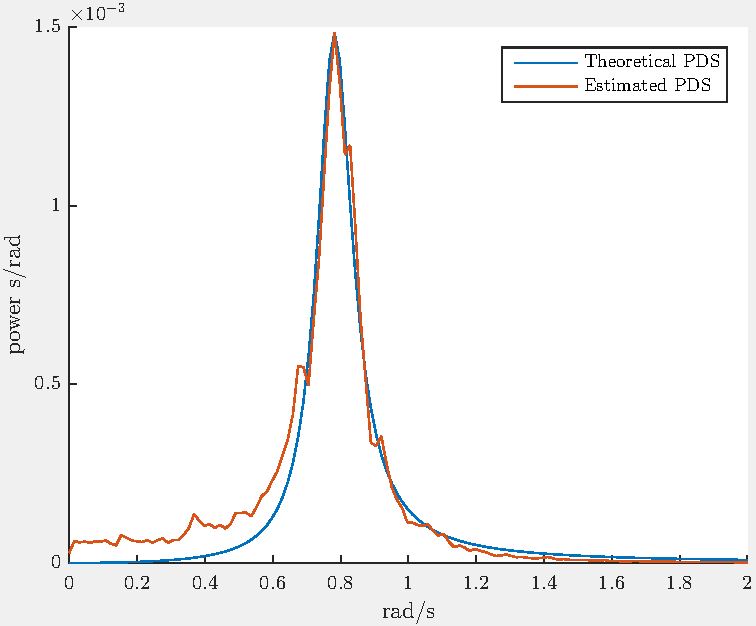
\includegraphics[width=0.5\textwidth]{images/2d-fitted_theoretical_PSD_vs_estimated_PSD}
    \caption{Fitted theoretical PSD vs estimated PSD}
    \label{fig:2d-fitted_theoretical_PSD_vs_estimated_PSD}
\end{figure}

\newpage
\section{Control system design}
\subsection{Problem a}

\todo{SPØR STUDASS HVORDAN man skal ta hensyn til $\psi$ i deloppgave b), c), og d). SVAR: Det er allerede tatt hensyn til ettersom psi holder seg innen 35 grader. Skriv om dette i svarene}


The PD transfer function is of the form
\begin{align*}
    H_{pd}(s) &= K_{pd}(1+T_d s)/(1+T_f s) \\
              &= K_{pd}(1+T s)/(1+\alpha T s)
\end{align*}

Where $T_d = T$ in order to cancel the systems pole factor $(Ts + 1)$, and $T_f = \alpha T_d = \alpha T$. We set $K_{pd} = 0.8, \alpha = 0.1$. \Cref{fig:3a-bode_and_phasemargin} contains the bode plot of the system $H(s) = H_{ship}(s)H_{pd}(s)$, with the phase margin Pm at 48.3 degrees, and crossover angular frequency at 0.104 rad/s.

Phase margin was found through the $margin(sys)$ MATLAB function, by using trial and error in placing $K_{pd}$ and $\alpha$. The $margin$ function calculates the phase margin by solving for the difference between the system phase and -180 degrees at the angular frequency where the systems amplitude is 1. \todo{Skriv litt bedre om margin funksjonen}

\begin{figure}[ht]
    \centering
    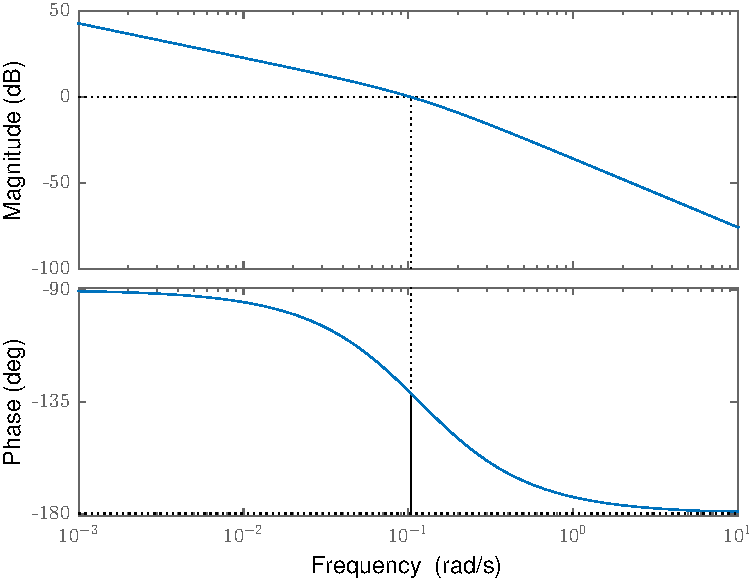
\includegraphics[width=0.5\textwidth]{images/3a-bode_and_phasemargin}
    \caption{Bode - and phase margin plot}
    \label{fig:3a-bode_and_phasemargin}
\end{figure}

\subsection{Problem b}
As shown in \cref{fig:3b-psi_and_rudder}, the autopilot functions well with only measurement noise.  It reaches the setpoint with acceptable inputs and minimal oscillations.

\begin{figure}[ht]
    \centering
    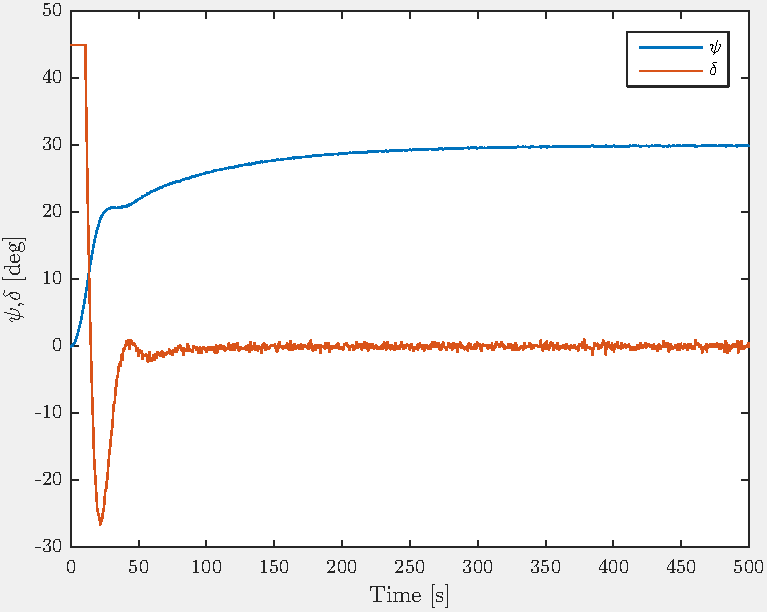
\includegraphics[width=0.5\textwidth]{images/3b-psi_and_rudder}
    \caption{Compass angle, $\psi$, and rudder angle, $\delta$, along the y-axis, plotted against time in the x-axis. With measurement noise}
    \label{fig:3b-psi_and_rudder}
\end{figure}

\subsection{Problem c}
With measurement noise and current disturbances, the autopilot functions as shown in \cref{fig:3b-psi_and_rudder_w_current}. While the angle approaches the setpoint with acceptable rudder inputs, there is an unacceptable steady state error, such that the angle never reaches the setpoint. This is expected since the current creates a bias in the rudder and there is no integral term in the controller to eliminate steady state errors.

\begin{figure}[ht]
    \centering
    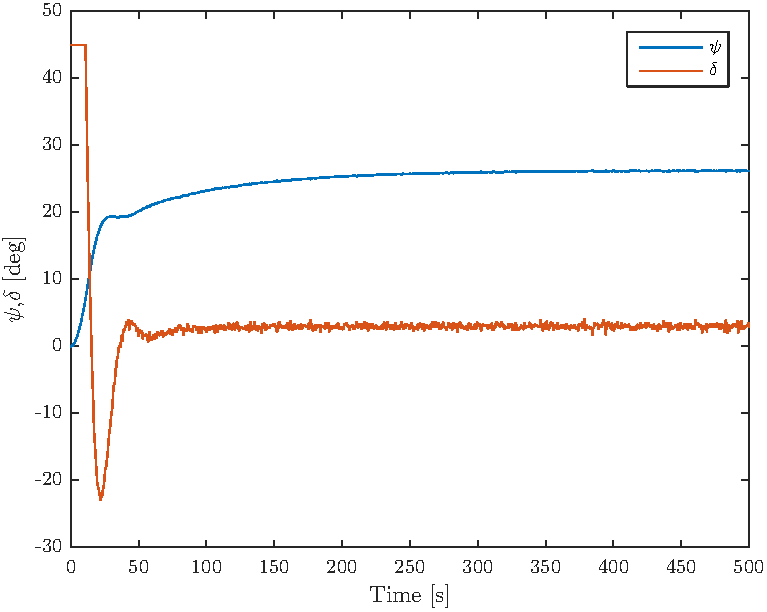
\includegraphics[width=0.5\textwidth]{images/3c-psi_and_rudder_w_current}
    \caption{Compass angle, $\psi$, and rudder angle, $\delta$, along the y-axis, plotted against time in the x-axis. With current disturbance and measurement noise}
    \label{fig:3b-psi_and_rudder_w_current}
\end{figure}

\subsection{Problem d}
With measurement noise, current and wave disturbances the autopilot functions as shown in \cref{fig:3b-psi_and_rudder_w_waves}. The controller reacts to the waves high frequency by creating unacceptable high frequency noise on the input. This would strain the motors and/or rudder of the ship. Furthermore, the heading does not settle on the setpoint, but rather oscillates around it in response to the waves. Since the disturbances are easily modeled, a filter could be used to reduce the noise in the controller. Therefore, the controller could better hold the ship's heading.

\begin{figure}[ht]
    \centering
    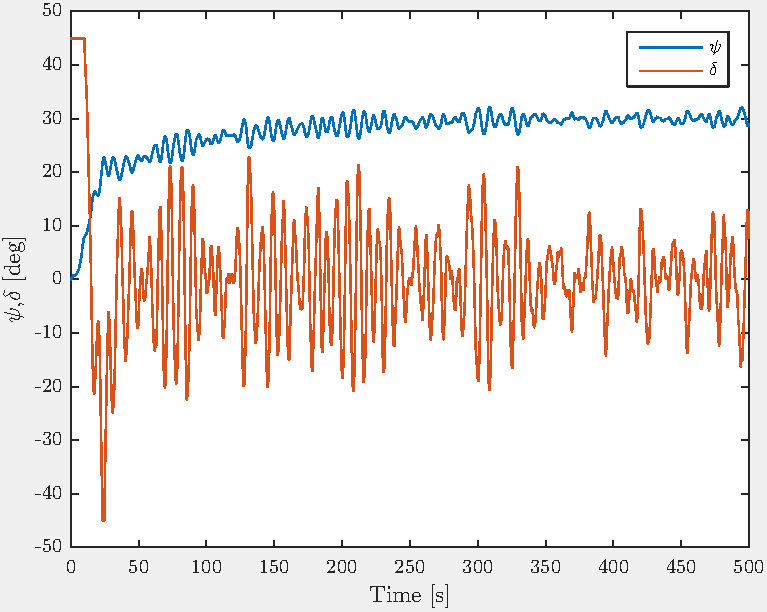
\includegraphics[width=0.5\textwidth]{images/3d-psi_and_rudder_w_waves}
    \caption{Compass angle, $\psi$, and rudder angle, $\delta$, along the y-axis, plotted against time in the x-axis. With wave disturbance and measurement noise}
    \label{fig:3b-psi_and_rudder_w_waves}
\end{figure}
\newpage
\section{Observability}
\subsection{Problem a}
The system described in equations 13a-13f \cite{assignment} can be described in state space form 
with state \textbf{x} = $[\xi_w\: \psi_w\: \psi\; r\: b]^T$, input $u = \delta$, 
disturbances \textbf{w} = $[w_w\: w_b]^T$ and output $y$:

\begin{align*}
    \bf{\dot{x}} &= \textbf{Ax} + \textbf{B}u + \textbf{Ew} \\
    \textbf{y} &= \textbf{Cx}
\end{align*}

with the matrices:

\begin{align*}
    A &= 
\end{align*}

\subsection{Problem b}
Uten disturbances
\subsection{Problem c}
current disturbance only
\subsection{Problem d}
wave disturbances
\subsection{Problem e}
both disturbances
\newpage
\section{Discrete Kalman filter}
\subsection{Discretization}
To design a discretized Kalman filter one must first discretize the system. For this discrete versions of $\bm{A}, \bm{B}, \bm{E}$ are required, in addition to discrete versions of the covariances of the disturbance $\bm{Q_w}$, and measurement noise $\bm{R_v}$.

The continuous solution of $\bm{x}$ with an input $\bm{u}$ with gain matrix $\bm{B}$, and disturbance $\bm{w}$ with gain matrix $\bm{E}$ is given by:
\begin{equation*}
\bm{x}(t) = e^{\bm{A}t}\bm{x}_0 + \int_0^te^{\bm{A}(t-\tau)}\bm{Bu}(\tau)d\tau + \int_0^te^{\bm{A}(t-\tau)}\bm{Ew}(\tau)d\tau
\end{equation*}
Using the continuous solution, we start it at $t=kT_s$ and stop it at $t=(k+1)T_s$. Here, $T_s = 1/F_s$ and $F_s = 10$ Hz is the sampling frequency. $T_s$ is thus the sampling period. Doing this, we get:
\begin{equation}
\bm{x}[k+1] = e^{\bm{A}T_s}\bm{x}_0 + \int_0^{T_s} e^{\bm{A}\alpha}\bm{Bu}((k+1)T_s -\alpha)d\alpha + \int_0^{T_s} e^{\bm{A}\alpha}\bm{Ew}((k+1)T_s -\alpha)d\alpha \label{x_disc}
\end{equation}

By setting a sampling period $T_s$ that is low enough, $\bm{u}$ and $\bm{w}$ can be seen as approximately constant between the time $t = kT_s$ and $t = (k+1)T_s$, and can be moved outside of our integral. Moving forward, $T_s$ is assumed to be low enough.

\begin{equation}
\bm{x}[k+1] = e^{\bm{A}T_s}\bm{x}_0 + \bm{u}\int_0^{T_s} e^{\bm{A}\alpha}\bm{B}d\alpha + \bm{w}\int_0^{T_s} e^{\bm{A}\alpha}\bm{E}d\alpha \label{x_disc_const}
\end{equation}

The exact discretized system is thus found to be:
\begin{subequations}
\begin{align}
    \dot{\bm{x}}[k+1] =& \ \thickbar{\bm{A}}\bm{x}[k]+\thickbar{\bm{B}}\bm{u}[k] + \thickbar{\bm{w}}[k], \\
    \thickbar{\bm{w}}[k] &= \thickbar{\bm{E}}\bm{w}[k], \label{w_bar} \\
    \thickbar{\bm{A}} &= e^{\bm{A}T_s}, \\
    \thickbar{\bm{B}} &= \int_{0}^{T_s}e^{\bm{A}\alpha}\bm{B}d\alpha \label{B_d}, \\
    \thickbar{\bm{E}} &= \int_{0}^{T_s}e^{\bm{A}\alpha}\bm{E}d\alpha \label{E_d}
\end{align}
\end{subequations}
The notation $\bm{X_d} = \thickbar{\bm{X}}$ is used in MATLAB code.

In MATLAB, they can be found through the
\texttt{[A$_d$\ B$_d$] = c2d(A, B, T$_s$)} function. \\ \texttt{c2d(A, B, T$_s$)} uses the Van Loan's method:
\begin{equation}
exp(
\begin{bmatrix}
\bm{A} & \bm{B} \\
\bm{0} & \bm{0} \\
\end{bmatrix}
T_s) = 
\begin{bmatrix}
\bm{N}_{11} & \bm{N}_{12} \\
\bm{0} & \bm{I} \\
\end{bmatrix}
,\ \thickbar{\bm{A}} = \bm{N}_{11},\  \thickbar{\bm{B}} = \bm{N}_{12}
\end{equation}
Since $\bm{w}$ can be seen as an input with gain matrix $\bm{E}$ of the continuous system, one can replace $\bm{B}$ with $\bm{E}$ in order to find $\thickbar{\bm{E}}$.

The autocovariance of $\thickbar{\bm{w}}$ is found through the following relations:

\begin{equation*}
    \thickbar{\bm{A}}_{\bm{w}}[k,l] = E((\thickbar{\bm{w}}[k]-\bm{m}_{\thickbar{\bm{w}}}[k])(\thickbar{\bm{w}}[l]-\bm{m}_{\thickbar{\bm{w}}}[l])^T)
\end{equation*}
Noting that the means are zero, and inserting the result into \cref{w_bar}, one finds:
\begin{align*}
    \thickbar{\bm{A}}_{\bm{w}}[k,l] &=
    E(\thickbar{\bm{E}}\bm{w}[k]\bm{w}[l]^T\thickbar{\bm{E}}^T) \\
    &= \thickbar{\bm{E}}E(\bm{w}[k]\bm{w}[l]^T)\thickbar{\bm{E}}^T \\
    &= \thickbar{\bm{E}}\bm{Q_w}\delta[k,l]\thickbar{\bm{E}}^T \\
    &= \thickbar{\bm{Q}}_{\bm{w}}\delta[k,l]
\end{align*}
Meaning the discretized $\thickbar{\bm{Q}}_{\bm{w}}$ is:
\begin{equation}
\thickbar{\bm{Q}}_{\bm{w}} =\thickbar{\bm{E}}\bm{Q}_{\bm{w}}\thickbar{\bm{E}}^T
\end{equation}
The discretized output of the system is:
\begin{equation*}
\bm{y}[k] = \bm{Cx}[k] + \thickbar{\bm{v}}[k]
\end{equation*}
where $\thickbar{\bm{v}}[k]$ is the averaged measurement noise. This is used as opposed to the direct measurement noise
at time $kT_s$ in order to avoid the exaggeration of sampling continuous time noise into discrete time.
\begin{equation*}
\thickbar{\bm{v}}[k] = \frac{1}{T_s}\int_{0}^{T_s}\bm{v}(kT-\alpha)d\alpha
\end{equation*}
The autocovariance of the noise becomes (again with mean equal to zero):
\begin{align*}
    \thickbar{\bm{A}}_\bm{v}[k, l] &= E(\thickbar{\bm{v}}[k]\thickbar{\bm{v}}[l]^T) \\
    &= \frac{1}{T_s^2}\int_{0}^{T_s}\int_{0}^{T_s}E(\bm{v}(kT_s-\alpha_1)\bm{v}(lT_s-\alpha_2)^T)d\alpha_1d\alpha_2 \\
    &= \frac{1}{T_s^2}\int_{0}^{T_s}\int_{0}^{T_s}\bm{R_v}\delta[k,l]\delta(\alpha_1-\alpha_2)d\alpha_1d\alpha_2 \\
    &= \frac{1}{T_s^2}\int_{0}^{T_s}\bm{R_v}\delta[k,l]d\alpha_1 \\
    &= \frac{1}{T_s}\bm{R_v}\delta[k,l] \\
    &= \thickbar{\bm{R}}_{\bm{v}}\delta[k,l]
\end{align*}
Meaning the discretized $\thickbar{\bm{R}}_{\bm{v}}$ is:
\begin{equation}
\thickbar{\bm{R}}_{\bm{v}} = \frac{\bm{R_v}}{T_s}
\end{equation}

\subsection{Measurement noise variance}
The ship system is simulated with a constant rudder $\delta$-input of 0 and only measurement noise turned on. An
estimate of the variance of 
the measurement noise is found by putting the compass output into the MATLAB function {\texttt{var(A)}}. This function
sums the squared distance of the values from the mean and divides this by the total number of values. The variance 
is found to be 0.0020.

\subsection{Implementation}
A discrete Kalman filter is to be designed. It is a discrete observer which performs optimal estimation through
minimizing the mean-square-error $J[k] = tr(\bm{P}[k])$, where
$\bm{P}[k] \triangleq E(\bm{e}[k]\bm{e}[k]^T) = E((\bm{x}[k] - \hat{\bm{x}}[k])(\bm{x}[k] - \hat{\bm{x}}[k])^T)$ is the
covariance matrix of the error between the states and the estimated states.

The estimate is generated in two phases, one guess for $\bm{x}[k]$ before $\bm{y}[k]$ is taken into account, called a
priori (prior observation), and one guess after called a posteriori (post observation).

A priori estimate:
\begin{equation}
\hat{\bm{x}}^-[k] = \thickbar{\bm{A}}\hat{\bm{x}}[k-1]+\thickbar{\bm{B}}\bm{u}[k-1] \label{a_priori_x}
\end{equation}
This is thus an a priori guess of the next $\hat{\bm{x}}[k]$ based on the previous a posteriori value of $\hat{\bm{x}}$ and the value of $\bm{u}$ at time k-1.

A posteriori estimate:
\begin{equation}
\thickbar{\bm{x}}[k] = \hat{\bm{x}}^-[k] + \bm{L}[k](\bm{y}[k] - \bm{C}\hat{\bm{x}}^-[k]) \label{a_posteriori_estimate}
\end{equation}
And this is the update of $\thickbar{\bm{x}}[k]$ based on the a priori value, the measured $\bm{y}[k]$, and the updated Kalman gain $\bm{L}[k]$.

With this, one can also define an a priori error and an a posteriori error, and an a priori and a posteriori covariance matrices. They are respectively:
\begin{align}
\bm{e}^-[k] &= \bm{x}[k] - \hat{\bm{x}}^-[k] \\
\bm{e}[k] &= \bm{x}[k] - \hat{\bm{x}}[k] \\
\bm{P}^-[k] &= E(\hat{\bm{x}}^-[k]\hat{\bm{x}}^-[k]^T) \\
\bm{P}[k] &= E(\hat{\bm{x}}[k]\hat{\bm{x}}[k]^T)
\end{align}

Using this information, one can find update rules for $\bm{P}^-[k], \bm{P}[k]$, and $\bm{L}[k]$. First we find update rules for the a priori and a posteriori error:
\begin{align*}
    \bm{e}^-[k] &= \bm{x}[k]-\hat{\bm{x}}^-[k] \\
                &= \thickbar{\bm{A}}\bm{x}[k-1] + \thickbar{\bm{B}}\bm{u}[k-1] + \thickbar{\bm{w}}[k-1] - (\thickbar{\bm{A}}\hat{\bm{x}}[k-1] + \thickbar{\bm{B}}\bm{u}[k-1]) \\
                &= \thickbar{\bm{A}}\bm{e}[k-1] + \thickbar{\bm{w}}[k-1] \\
    \bm{e}[k]&= \bm{x}[k] -\hat{\bm{x}}[k] \\
             &= \bm{x}[k] - (\bmhat{x}^-[k]+\bm{L}[k](\bm{y}-\bm{C}\bmhat{x}^-[k])) \\
             &= \bm{x}[k] - (\bmhat{x}^-[k]+\bm{L}[k](\bm{C}\bm{x}[k] -\bm{C}\bmhat{x}^-[k]+\bmbar{v}[k])) \\
             &= \bm{e}^-[k] - \bm{L}[k]\bm{C}\bm{e}^-[k]-\bm{L}[k]\bmbar{v}[k]
\end{align*}
The a priori covariance matrix becomes:
\begin{align*}
    \bm{P}^-[k] &= E(\bm{e}^-[k]\bm{e}^-[k]^T) \\
                &= E((\thickbar{\bm{A}}\bm{e}[k-1] + \thickbar{\bm{w}}[k-1])(\thickbar{\bm{A}}\bm{e}[k-1] + \thickbar{\bm{w}}[k-1])^T) \\
                &= \thickbar{\bm{A}}E(\bm{e}[k-1]\bm{e}[k-1]^T)\thickbar{\bm{A}}^T + E(\thickbar{\bm{w}}[k-1]\thickbar{\bm{w}}[k-1]^T)
\end{align*}
The last line follows because $\bm{e}$ and $\bm{w}$ are uncorrelated. This simplifies to
\begin{equation}
\bm{P}^-[k] = \thickbar{\bm{A}}\bm{P}[k-1]\thickbar{\bm{A}}^T + \thickbar{\bm{Q}}_{\bm{w}} \label{a_priori_covariance}
\end{equation}

And the a posteriori covariance matrix becomes:
\begin{align*}
    \bm{P}[k] &= E(\bm{e}[k]\bm{e}[k]^T) \\
              &= E(\ ((\bm{I} - \bm{L}[k]\bm{C})\bm{e}^-[k]+\bm{L}[k])((\bm{I} - \bm{L}[k]\bm{C})\bm{e}^-[k]+\bm{L}[k])^T) \\
              &= (\bm{I} - \bm{L}[k]\bm{C})E(\bm{e}^-[k]\bm{e}^-[k]^T)(\bm{I} - \bm{L}[k]\bm{C})^T + \bm{L}[k]\bmbar{R}_{\bm{v}}\bm{L}[k]^T
\end{align*}
Again, where the last line follows because $\bm{e}^-[k]$ and $\bmbar{v}$ are uncorrelated. The result:
\begin{equation}
              \bm{P}[k] = (\bm{I} - \bm{L}[k]\bm{C})\bm{P}^-[k](\bm{I} - \bm{L}[k]\bm{C})^T + \bm{L}[k]\bmbar{R}_{\bm{v}}\bm{L}[k]^T \label{a_posteriori_covariance}
\end{equation}

Lastly, one can now find the update rule for $\bm{L}[k]$. This is the Kalman gain, and it functions as a gain to $\bm{y}$ and the estimated $\bmhat{y} = \bm{C}\bmhat{x}$. It is selected in order to minimize the error between them. The Kalman gain $\bm{L}[k]$ is found by minimizing the mean-square-error $J[k] = tr(\bm{P}[k])$ with respect to $\bm{L}[k]$, i.e $\frac{\partial tr(\bm{P}[k])}{\partial\bm{L}[k]} = \bm{0}$. The result:
\begin{equation}
\bm{L}[k] = \bm{P}^-[k]\bm{C}^T(\bm{CP}^-[k]\bm{C}^T+\bmbar{R}_{\bm{v}})^{-1} \label{kalman_update}
\end{equation}

And with all that, the Kalman filter can be designed. It performs the following calculations in the following order:
\begin{enumerate}
 \item $\bmhat{x}^-[0]$ and $\bm{P}^-[0]$ are initialized to $E(\bm{x}[0]) = \bm{m}_{\bm{x}_0}$ and $E(\bm{e}^-[0]\bm{e}^-[0]^T) = \mathcal{C}_{\bm{x}_0}$ respectively.
 \item The update of the Kalman gain is performed using  \cref{kalman_update}.
 \item The a posteriori estimate of the states is calculated using  \cref{a_posteriori_estimate}.
 \item The error covariance matrix is updated using  \cref{a_posteriori_covariance}.
 \item The a priori values of $\bmhat{x}^-$ and $\bm{P}^-$ are found for the next time step $k+1$, using \cref{a_priori_x} and \cref{a_priori_covariance}.
 \item Start from step 2 again for the next time step $k+1$.
\end{enumerate}

This was implemented in simulink using zero-order hold blocks to discretize to system by holding the values for each time step, and memory blocks to hold the previous a priori values first initialized in step 1, and updated in step 5 above. The updates were implemented as function blocks, and the updates themselves were thus written as MATLAB functions. These can be seen in \cref{sec:Appendix A}.

\subsection{Feed forward from estimated bias}
The Kalman filter gives access to an estimate of the bias to the rubber angle (\cref{fig:5d-estimated_rudder_bias}).  With current disturbance on, this bias became apparent as a steady-state error when attempting to steer the ship (Part 3.3 \cref{fig:3b-psi_and_rudder_w_current}).  However, this bias can now be compensated for by adding the estimated bias as a feedforward term to the rudder input.  The results of using this term, with current disturbances on, is seen in \cref{fig:5d-psi_and_rudder}.  This term removes the steady state error seen previously, which is a significant improvement. Again, $\psi$ is within the boundary of $\pm35$, so the ship model holds.

\begin{figure}[h!]
    \centering
    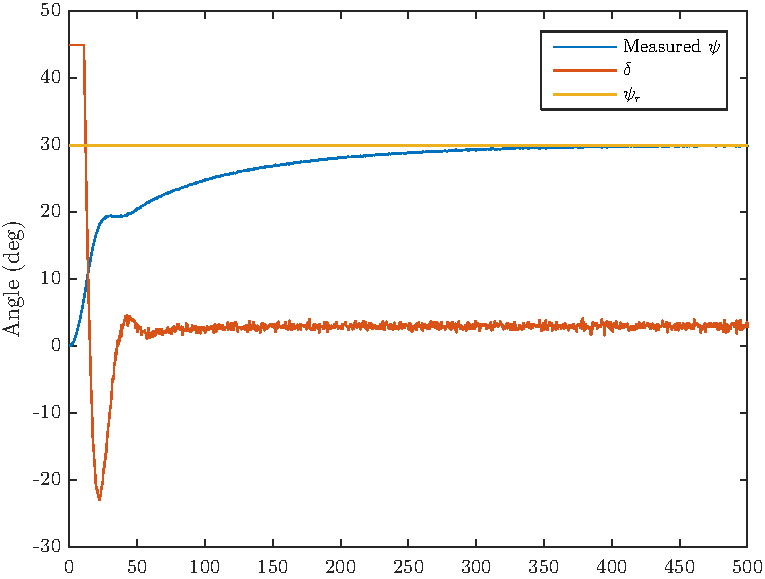
\includegraphics[width=0.5\textwidth]{images/5d-psi_and_rudder}
    \caption{Compass angle, $\psi$, and rudder angle, $\delta$, along the y-axis, plotted against time in the x-axis. Using estimated bias from \cref{fig:5d-estimated_rudder_bias} as feedforward term added to the rudder input. With current disturbance and measurement noise}
    \label{fig:5d-psi_and_rudder}
\end{figure}

\begin{figure}[h!]
    \centering
    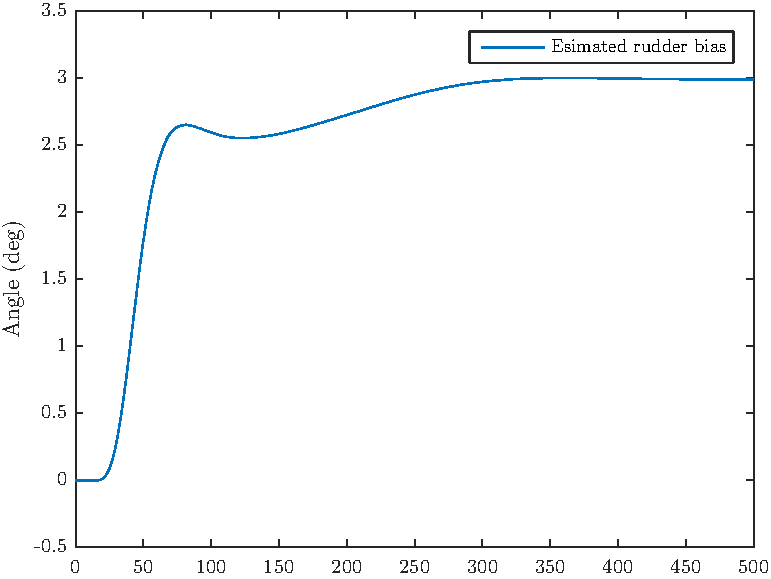
\includegraphics[width=0.5\textwidth]{images/5d-estimated_rudder_bias}
    \caption{Kalman estimated rudder bias over time. With current disturbance and measurement noise}
    \label{fig:5d-estimated_rudder_bias}
\end{figure}

\subsection{Wave filtering}
The Kalman filter also gives access to a filtered estimate of the compass heading. This reduces the high frequency noise due to the waves on the compass heading. The results of simulating the ship using the filtered estimate for $\psi$ as the input to the controller is shown in \cref{fig:5e-psi_and_rudder}. The estimated compass angle does not have large oscillations compared to the measured compass angle. This leads to reasonable rudder inputs and roughly the same output from the controller as the same simulation with the measured compass angle used as feedback (Part3D \cref{fig:3b-psi_and_rudder_w_waves}). Using the inputs from the previous simulation would possibly break the rudder or its motor or at least cause significant strain, while these inputs are much more tame and smooth, which is a significant improvement. Once again, $\psi$ is within the boundary of $\pm35$, so the ship model holds.

\begin{figure}[htp]
    \centering
    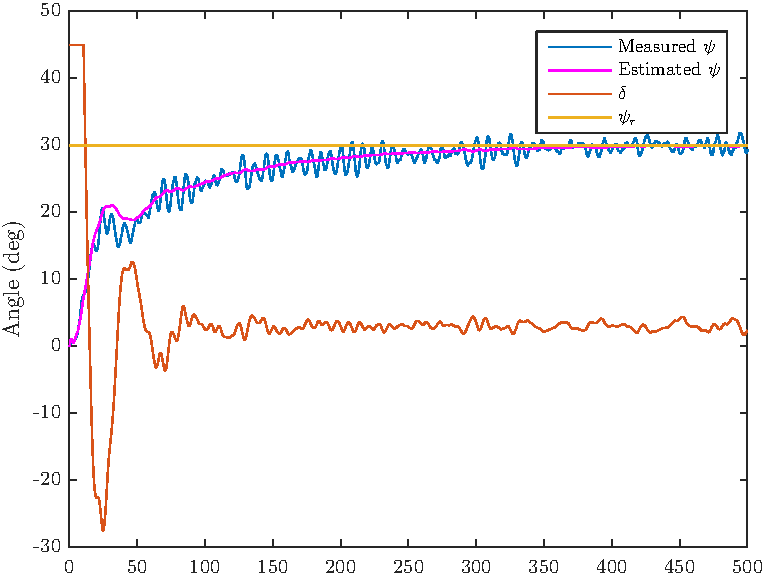
\includegraphics[width=0.5\textwidth]{images/5e-psi_and_rudder}
    \caption{Compass angle, $\psi$, and rudder angle, $\delta$, along the y-axis, plotted against time in the x-axis. Using estimated compass angle as feedback to the controller. With current and wave disturbances and measurement noise}
    \label{fig:5e-psi_and_rudder}
\end{figure}

\begin{figure}[htp]
    \centering
    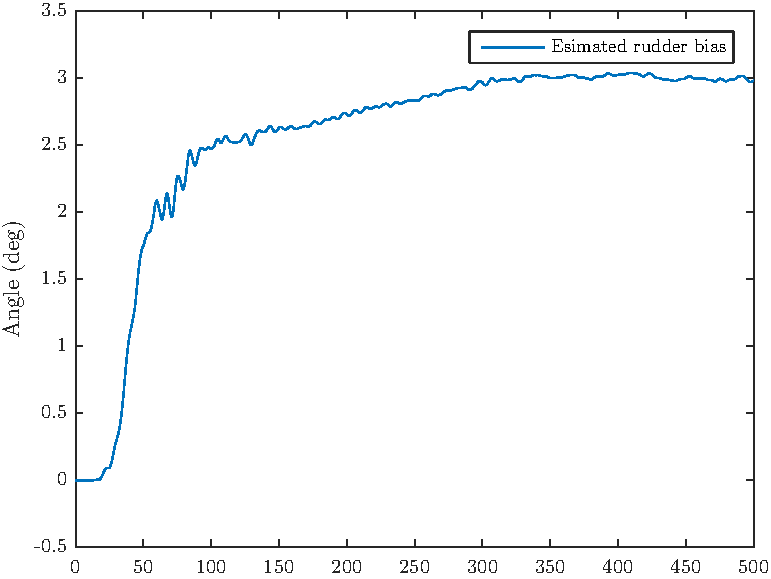
\includegraphics[width=0.5\textwidth]{images/5e-estimated_rudder_bias}
    \caption{Kalman estimated rudder bias over time. With current and wave disturbances and measurement noise}
    \label{fig:5e-estimated_rudder_bias}
\end{figure}

The wave noise estimate follows the pattern of the actual waves, but is quite damped in comparison.  This points to a likely error in the Kalman filter. This error is most likely a mismatched unit, for example degrees instead of radians, and could also explain why the estimated compass angle oscillates around the measured value slightly and the rudder bias oscillates before settling at 3 degrees.  These oscillations seem to be exacerbated by large changes in the measured value, meaning the the Kalman gains are too small, thereby over-prioritizing the current estimated state compared to the new measurements. This can be due to error(s) in the calculation or update of the P matrix, which in turn could be due to the measurement variance or the discretized A or Q matrices.

\begin{figure}[htp]
    \centering
    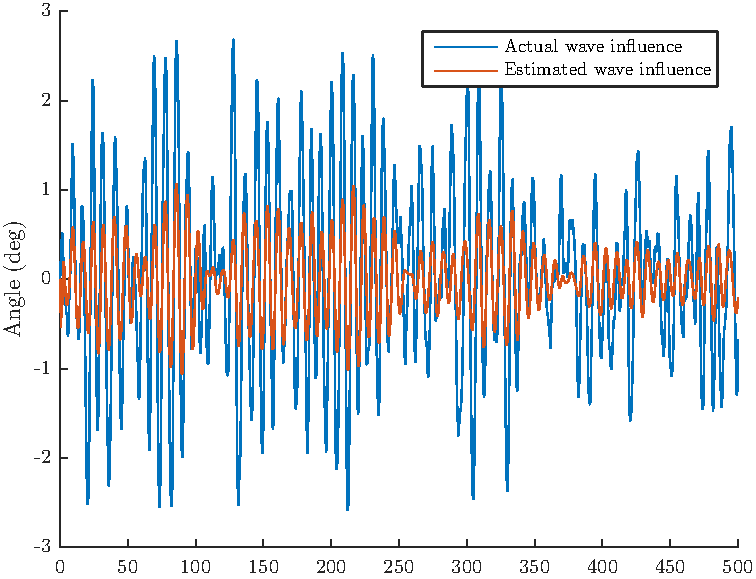
\includegraphics[width=0.5\textwidth]{images/5e-wave_influence}
    \caption{Estimated wave noise versus actual wave noise.}
    \label{fig:5e-wave_influence}
\end{figure}

In order to improve upon this result, there are a number of things that could be done.
\begin{itemize}
    \item $T_s$ could be made even smaller - a smaller sampling time could discretize the system better. Due to the high variation of the waves $T_s$ needs to be sufficiently small in order to ensure the assumption that $w_w$ is constant over the integration period holds.
    \item The controller could be tuned to reduce large swings in the input, which lead to large changes in the state that are difficult for the filter to detect. 
    \item Tune the filter so that it reacts better to large quick changes in state. This is done through tuning the $\bmbar{Q}_{\bm{w}}$ and $\bmbar{R}_{\bm{v}}$ matrices, as they function like LQR Q and R matrices.

\end{itemize}
\newpage
\begin{thebibliography}{9}
\bibitem{chen14}
  Chi-Tsong Chen,
  \emph{Linear System Theory and Design},
  Oxford University Press,
  4th edition,
  2014
\end{thebibliography}
\end{document}